\documentclass{beamer}
\usepackage{graphicx}
\usepackage{float}
\usepackage{amsmath}
\usetheme{Madrid}
\usecolortheme{seahorse}
%Information to be included in the title page:
\title[MC758] %optional
{Teoria dos Jogos}

\subtitle{Mecanismos de aproximação computacionalmente eficientes}

\author[Radeck] % (optional, for multiple authors)
{R.~Radeck}

\institute[IC] % (optional)
{
  Instituto de Computação\\
  Universidade estadual de Campinas
}

\date[] % (optional)
{Novembro de 2022}

\graphicspath{ {images/} }

\begin{document}

\frame{\titlepage}

\begin{frame}
    \frametitle{Introdução - Algoritmos vs Mecanismos}
    Apesar de algoritmos e mecanismos terem uma natureza muito próximas, a maneira que cada técnica é utilizada na resolução de problemas é diferente. %\pause

    \begin{itemize}
        \item{Mecanismos: Formulação complexa e muitas soluções técnicas para os designs clássicos, porém ineficientes computacionalmente.} %\pause

        \item{Algoritmos: Em geral trabalham muito bem com perguntas computacionais, porém não funcionam bem com as necessidades dos mecanismos da teoria dos jogos.} %\pause
    \end{itemize}
    
    Como podemos ver existe um impasse natural sobre esses temas e aqui vamos ver a melhor maneira de extrair o ótimo de cada técnica computacional para cada tipo de mecanismo.
\end{frame}

\begin{frame}
    \frametitle{Introdução - Dividindo os Mecanismos}
    Vamos separar nossos mecanismos de acordo com a dimensionalidade de seus domínios, já que isso está fortemente atrelado a eficiência e outras propriedades computacionais deles. %\pause

    \begin{itemize}
        \item{Em mecanismos unidimensionais garantir monotonicidade algorítimica é suficiente para que a veracidade da teoria dos jogos seja garantida, o que nos dá bastante flexibilidade para elaboração de algoritmos.} %\pause
        \item{Porém, em mecanismos multidimensionais, algumas dificuldades surgem. Aqui vamos analisar além da monotonicidade na construção de algoritmos determinísticos, soluções que apresentam fatores aleatórios que nos ajudarão a superar essas dificuldades e vamos também considerar noções alternativas sobre o conceito de veracidade.}
    \end{itemize}
        
\end{frame}

\begin{frame}
    \frametitle{Mecanismos Unidimensionais - Balanceamento de Carga}
    Vamos trabalhar com o exemplo de máquinas relacionadas para nosso domínio unidimensional. Nesse quesito, $n$ tarefas precisam ser alocadas em $m$ máquinas, onde a tarefa $j$ consome $p_j$ unidades de tempo e a máquina $i$ tem velocidade $s_i$. Dessa forma a máquina $i$ demora $p_j/s_i$ unidades de tempo para completar o trabalho $j$. Seja $l_i$ a carga ($\sum{p_j}$ para todo $j$ relacionado para $i$) da máquina $i$, nosso objetivo é minimizar $\max{l_i/s_i}$ (minimizar o \textit{makespan}). Como cada máquina é uma entidade egoísta e quer maximizar sua utilidade (diminuir seu custo), isso faz com que exista um custo constante para cada unidade de tempo consumida. Portanto a utilidade de uma máquina $i$ será $-l_i/s_i - P_i$, onde $P_i$ é o pagamento da máquina.
\end{frame}

\begin{frame}
    \frametitle{Mecanismos Unidimensionais - Unidimensionalidade}
    Se não conseguimos separar nossas alternativas em ``perder'' e ``ganhar'', porquê esse exemplo é unidimensional? Vamos analisar a definição. %\pause

    \begin{block}{Domínios unidimensionais e lineares}
        Um domínio $V_i$ de um jogador $i$ é unidimensional e linear se existem constantes reais e não negativas (as ``cargas'') $\left\{q_{i, a}\right\}_{a \in A}$ tal que, para toda jogada $v_i \in V_i$, existe $c$ (o ``custo'') também real e não negativo tal que $v_i(a) = q_{i, a} \cdot c$.
    \end{block} %\pause
    Note que o domínio da atribuição de um jogador é de fato unidimensional e linear, já que o parâmetro $c$ é igual a $1/s_i$, e a constante $q_{i, a}$ para a atribuição $a$ é a carga $l_i$ da máquina $i$, de acordo com aquela atribuição.
\end{frame}

\begin{frame}
    \frametitle{Mecanismos Unidimensionais - Implementabilidade}
    Precisamos agora garantir a implementabilidade de um algoritmo para mecanismos de domínio unidimensionais e lineares. Como nosso domínio é convexo, fixando $c_{-i}$ e tomando $c' > c$, onde $c$ é o custo dado pelo jogador $i$, nós precisamos garantir apenas que $-q_i(c')(c' - c) \geq$ $-q_i(c)(c' - c)$, ou seja, que $-q_i(c') \geq -q_i(c)$. (``Monotonicidade fraca'')
    
    \begin{figure}[H]
        \centering
        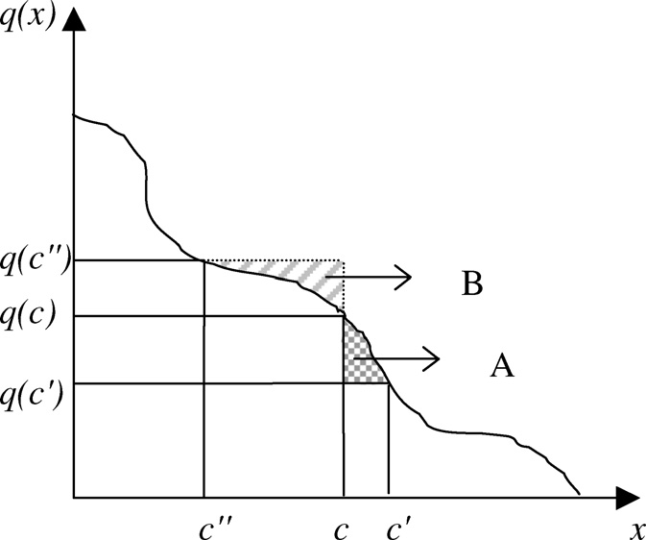
\includegraphics[width=0.4\textwidth]{image1.png}
        \\{Curva monotônica de carga}
    \end{figure} 
\end{frame}

\begin{frame}
    \frametitle{Mecanismos Unidimensionais - Implementabilidade}
    Suponha que a cobrança seja $P_i(c) = \int_{0}^{c} \left(q_i(x) - q_i(c) \right) \delta x$, ou seja, a área abaixo da curva da figura anterior. Observando atentamente, vemos que não é vantajoso para o jogador declarar um custo diferente de $c$, já que qualquer outro valor declarado resultará em mudanças no valor da carga (diminui se $c$ aumenta) e no valor da cobrança (diminui se o $c$ diminui), resultando em percas no valor das áreas apresentadas na imagem. Sendo assim esses preços satisfazem as inequações de incentivo-compatibilidade, e de fato é uma prova simples e direta para a suficiência monotônica de cargas nesse caso. Porém esses preços não incentivam uma jogada correta já que sempre os jogadores terão utilidade negativa (mesmo se tiverem carga 0).
\end{frame}

\begin{frame}
    \frametitle{Mecanismos Unidimensionais - Implementabilidade}
    Para resolver isso devemos acrescentar uma constante grande o suficiente aos preços, que nesse caso pode ser a área total da curva $\int_{0}^{\infty} q_i(x) \delta x$. Isso é uma boa escolha já que aqueles jogadores que declaram custo infinito (carga 0), terão utilidade 0 e em geral a utilidade de um jogador verdadeiro será não negativa, $\int_{c}^{\infty} q_i(x) \delta x$. Portanto, %\pause
    \begin{block}{Teorema}
        Um algoritmo para um domínio linear e unidimensional é implementável se e somente se suas funções de carga são não crescentes. Além disso, o preço cobrado de cada jogador será
        $$
        P_i(c) = \int_{0}^{c} \left(q_i(x) - q_i(c) \right) \delta x - \int_{c}^{\infty} q_i(x) \delta x
        $$
        resultando em uma implementação de uma estratégia dominante e individualemnte racional.
    \end{block}
\end{frame}

\begin{frame}
    \frametitle{Mecanismos Unidimensionais - Implementação}
    Agora nós devemos construir um algoritmos para resolver o problema do balanceamento de carga. Na verdade é até possível construir um algoritmo que nos retorna uma solução ótima, porém ele é da classe NP-Difícil e nós desejamos construir um algoritmo eficiente, sendo assim, um algoritmo monotônico e polinomial. Primeiramente vamos assumir os seguintes pontos:
    \begin{itemize}
        \item{$s_1 \geq s_2 \geq \cdots \geq s_m$}
        \item{$p_1 \geq p_2 \geq \cdots \geq p_n$}
    \end{itemize}
    Como o algoritmo que vamos projetar é monotônico, precisamos estimar um \textit{makespan} ótimo.
\end{frame}

\begin{frame}
    \frametitle{Mecanismos Unidimensionais - Implementação}
    Vamos fixar uma tarefa $j$ e um \textit{makespan} alvo $T$. Se uma atribuição tem \textit{makespan} menor ou igual a T, então essa atribução deve relacionar qualquer tarefa $\in \{1, 2, \ldots, j\}$ em alguma máquina, de tal forma que aquela máquina não demore mais que T para completar, ou seja, $T \geq p_j/s_i$. Seja $i(j, T)$ a máquina mais a direita (maior índice - menor velocidade) tal que $T \geq p_j/s_i$. Então nossa atribuição deve relacionar as tarefas de 1 a $j$ com as máquinas de 1 a $i(j, T)$. Temos então que:
    $$
        T \geq \frac{\sum_{k = 1}^{j} p_k}{\sum_{l = 1}^{i(j, T)} s_l}
    $$
    E vamos definir
    $$
        T_j = min \left[ max\left( \frac{p_j}{s_i}, \frac{\sum_{k = 1}^{j} p_k}{\sum_{l = 1}^{i} s_l} \right) \right] \forall i
    $$
\end{frame}

\begin{frame}
    \frametitle{Mecanismos Unidimensionais - Implementação}
    Note que o termo esquerdo cresce com $i$ e o direito decresce, isso nos permite mostrar que para qualquer $j$, o \textit{makespan} ótimo é pelo menos $T_j$, já que se existisse $T < T_j$, violaria o fato de ser um domínio unidimensional e linear. Seja $i_j$ o índice determinado por $T_j$, utilizando o fato que nossa função de máximo tem um ponto de virada, $i_j$ é um dos dois pontos onde ocorre a transição, podemos mostrar que em qualquer um desses pontos $T$ violaria nossa condição.

    Finalmente podemos definir a nossa estimativa para o \textit{makespan} ótimo sendo
    $$
        T_{LB} = max_j T_j
    $$
    Já que o ótimo é pelo menos $T_j$ para todo $j$, ele é pelo menos $T_{LB}$. 
\end{frame}

\begin{frame}
    \frametitle{Mecanismos Unidimensionais - Implementação}
    Vamos considerar o nosso problema com um relaxamento, as tarefas podem ser divididas em máquinas diferentes. Seja $j$ a primeira tarefa que quando colocada com as anteriores a ela na máquina 1, exceda o limite do nosso $makespan$, ou seja $\sum_{k = 1}^{j} > T_{LB} \cdot s_1$. Coloque as tarefas $1, 2, \ldots, j - 1$ e uma fração da tarefa $j$ na máquina 1 de tal forma que $l_1 = T_{LB} \cdot s_1$. Continue com as frações e máquinas restantes recursivamente. 

    Isso de fato é ótimo para não excedermos o limite de $T_{LB}$, mas como sabemos que não vai sobrar nenhuma fração de nenhuma tarefa? Veja que
    $$
        T_{LB} \geq T_j \geq \frac{\sum_{k = 1}^{j} p_k}{\sum_{l = 1}^{i_j} s_l}
    $$
    para todo $j$, então se $j = n$, fica trivial ver esse fato.
\end{frame}

\begin{frame}
    \frametitle{Mecanismos Unidimensionais - Implementação}
    Agora vamos considerar o caso geral, cada tarefa tem que ser alocada para exatamente uma máquina. Observe que a partir do caso fracionário, cada máquina vai receber o resto de uma fração que está lá, ou dar essa fração para a máquina que está com a outra parte da fração (a anterior ou a próxima). Assim nós vamos analisar dois casos e aqui que nós teremos a união entre algoritmos e mecanismos. O primeiro caso será uma escolha randômica deonde cada fração irá e isso nos fornece uma 2-aproximação (isso porquê a função de carga fracional é monotônica), porém viola o fato da monotonicidade. O segundo caso será um algoritmo determinístico que usa de conceitos mais fortes sobre a veracidade e mantém a monotonocidade, porém obtém uma aproximação pior.
\end{frame}

\begin{frame}
    \frametitle{Mecanismos Unidimensionais - Implementação Randômica}
    \begin{block}{Algoritmo randômico}
        Dado um $\alpha \in [0, 1]$ escolhido de maneira aleatória e uniforme, para cada tarefa $j$ que teve suas frações relacionadas com as máquinas $i$ e $i + 1$, se a fração em $i$ é pelo menos $\alpha$, relacione $j$ inteiramente com $i$, caso contrário, relacione $j$ inteiramente com $i + 1$.
    \end{block}
    Vamos verficar a aproximação. A partir do caso fracional, uma máquina $i$ pode aumentar seu número de trabalhos inteiros em no máximo 2, receber a fração da máquina imediatamente antes ($i - 1$) e da imediatamente depois ($i + 1$), sejam essas tarefas $j$ e $k$ respectivamente. De $j$, $p_i$ aumenta em no máximo $\alpha \cdot p_j$, da mesma forma de $k$, $p_i$ aumenta em no máximo $(1 - \alpha) \cdot p_k$ e como $\max\{p_j, p_k\} \leq T_{LB} \leq T_{opt}$. E qual a fração esperada em $i$? $1 - \alpha (j) + \alpha (k)$, ou seja, exatamente a esperada no caso fracionário.
\end{frame}

\begin{frame}
    \frametitle{Mecanismos Unidimensionais - Implementação Determinística}
    \begin{block}{Algoritmo determinístico}
        \begin{enumerate}
            \item{Crie velocidades virtuais para cada máquina $d_1, d_2, \ldots, d_m$. Seja $d_1 = \frac{8}{5}s_1$ e para qualquer $i > 1$, $d_i$ será o valor mais próximo dos valores \{$\frac{s_1}{2,5^i}, i = 1, 2, \ldots $\}, e $d_i \leq s_i$.}
            \item{Calcule o novo valor de $T_{LB}$ com as velocidades virtuais.}
            \item{Faça a atribuição das tarefas, começando da maior tarefa e da máquina mais rápida. Vá para a próxima máquina quando a atual ($i$), estiver com um tempo de processamento maior ou igual a $T_{LB} \cdot d_i$}
        \end{enumerate}
    \end{block}
    Note que se a priemira máquina muda de velocidade, todas as outras também mudam (virtualmente), além disso estamos fazendo uma atribuição de modo determinístico o que nos permite manter a monotonicidade, porém com uma perda de aproximação (fator de 5).
\end{frame}

\begin{frame}
    \frametitle{Mecanismos Multidimensionais}
    Como mencionado previamente, os mecanismos de domínio multidimensional são muito mais difíceis de serem considerados implementáveis, devido a complexidade das condições de monotonicidade para esses mecanismos. Para superar essas dificuldades, utilizaremos principalmente de técnicas de aleatorização. Vamos então considerar em nosso mecanismo exemplo Leilões Combinatórios. Esse tipo de mecanismo aparece muito frequentemente em problemas reais e é muito importante que existam algoritmos eficientes que consigam resolver esses problemas de maneira rápida.
\end{frame}

\begin{frame}
    \frametitle{Mecanismos Multidimensionais - Leilão Combinatório}
    Vamos relembrar os principais pontos de um Leilão combinatório:
    \begin{itemize}
        \item{Um conjunto de $m$ itens. ($\Omega$)}
        \item{Um conjunto de $n$ jogadores.}
        \item{Cada jogador possui uma função de valor $v_i(S)$, onde $S \subseteq \Omega$}
        \item{Funções de valor são monotônicas ($v_i(S) \leq v_i(T) \Leftrightarrow S \subseteq T$) e normalizadas ($v_i(\emptyset) = 0$)}
    \end{itemize}
    O objetivo é maximizar o bem-estar social, ou seja, encontrar uma alocação (atribuição) $S = (S_1, S_2, \ldots, S_n)$ que maximiza $\sum_{i}{v_i(S_i)}$. Vale lembrar que uma análise ingênua vai ter uma entrada de dados exponencial e que é NP-Difícil encontrar uma aproximação determinística com fator melhor que $\sqrt{m}$.
\end{frame}

\begin{frame}
    \frametitle{Mecanismos Multidimensionais - Leilão Combinatório}
    Vamos descrever nosso problema de forma mais geral como um programa linear, assim vamos converter um dado algoritmo para o problema de LC para uma \textit{c}-aproximação ao bem-estar social fracionário ótimo, isso com ajuda de técnicas de aleatorização. Para elaborarmos isso de maneira mais formal, vamos separar em 3 passos.
    \begin{itemize}
        \item{Domínio fracional.}
        \item{Como converter isso para o domínio original sem perda de veracidade.}
        \item{Técnica de decomposição.}
    \end{itemize}
\end{frame}

\begin{frame}
    \frametitle{Mecanismos Multidimensionais - Domínio Fracional}
    Seja $x_{i, S}$ a fração do subconjunto $S$ que o jogador $i$ recebe na alocação $x$, podemos assumir que o valor daquela fração é $v_i(S) \cdot x_{i, S}$. Assim nosso programa linear fica definido da seguinte forma:
    $$
        \textrm{max } \sum_{i, S \neq \emptyset} x_{i, S} \cdot v_i(S)
    $$$$
        \textrm{sujeito a } \sum_{S \neq \emptyset} x_{i, S} \leq 1 \textrm{ para cada jogador } i
    $$$$
        \sum_i \sum_{S: j \in S} x_{i, S} \leq 1 \textrm{ para cada item } j
    $$$$
        x_{i, S} \geq 0 \textrm{    } \forall i, S \neq \emptyset
    $$
\end{frame}

\begin{frame}
    \frametitle{Mecanismos Multidimensionais - Domínio Fracional}
    De acordo com a segunda restrição, cada jogador recebe no máximo um subconjunto inteiro e a terceira nos garante que um item não será alocado para mais de um jogador.

    Observe que esse programa linear pode ser resolvido em tempo polinomial de acordo com o seu tamanho e isso vai depender de qual linguagem vamos escolher para representar nosso leilão. Se utilizarmos linguagens de oferta nosso LP vai ter tamanho polinimial de acordo com o tamanho da oferta. Se utilizarmos uma linguagem de acesso a consulta, nosso LP será polinomial de acordo com a quantidade de consultas. Em ambos os casos a quantidade de coordenadas $x_{i, S} \neq 0$ é polinomial, já que $x$ é obtido em tempo polinimial. Além disso podemos utilizar VCG para obter uma alocação ótima.
\end{frame}

\begin{frame}
    \frametitle{Mecanismos Multidimensionais - Transição para inteiros}
    Vamos primeiro decompor nosso domínio fracional em pontos consideráveis e inteiros para o LP
    \begin{block}{Definição}
        Um algoritmo A verifica uma ``\textit{c}-integralidade'' para nosso LP se este recebe uma entrada com números reais $w_{i, S}$ e retorna um ponto inteiro $\tilde{x}$ que é considerável para o LP e 
        $$
            c \cdot \sum_{i, S} w_{i, S} \cdot \tilde{x}_{i, S} \geq \max_{\textrm{x considerável}} \sum_{i, S} w_{i, S} \cdot x_{i, S}
        $$
    \end{block}
    \begin{block}{Lema da decomposição}
        Se A verifica a ``\textit{c}-integralidade'' para um LP em tempo polinomial e $x$ é algum ponto que pode ser considerado pelo LP. Então pode-se decompor $x/c$ em uma combinação convexa e pontos inteiros e consideráveis em tempo polinomial.
    \end{block}
\end{frame}

\begin{frame}
    \frametitle{Mecanismos Multidimensionais - Transição para inteiros}
    Agora vamos nos preocupar em como retornar ao caso inteiro sem perder a veracidade a partir da decomposição obtida. Isso será feito utilizando aleatoriedade da seguinte maneira:

    Sejam $\{x^l\}_{l \in L}$ todas as atribuições inteiras. Nó vamos encontrar $\{\lambda_l\}_{l \in L}$, de tal forma que $\forall l \in L$, $\lambda_l \geq 0$, $\sum_{l \in L} \lambda_l = 1$ e $\sum_{l \in L} \lambda_l \cdot x^l = \frac{x}{c}$.
    \begin{block}{Mecanismo de decomposição}
    \begin{enumerate}
        \item{Calcule a solução fracionária ótima, $x^*$ e os preços de VCG $p_i^F(v)$.}
        \item{Calcule a decomposição $x^*/c = \sum_{l \in L} \lambda_l$.}
        \item{Com probabilidade $\lambda_l$, escolha uma alocação $x^l$, defina os preços $p_i^R(v) = \left( \frac{v_i(x^l)}{v_i(x*)} \right) \cdot p_i^F(v)$.}
    \end{enumerate}
    \end{block}
\end{frame}

\begin{frame}
    \frametitle{Mecanismos Multidimensionais - Transição para inteiros}
    As proposições estratégicas desse mecanismo funcionam sempre que os preços esperados são os mesmos que o preço fracional sobre $c$. Os preços são escolhidos especificamente para satisfazer, além das proposições estratégicas, uma racionalidade individual forte (encoraja que os jogadores falem a verdade, garantindo uma utilidade não negativa se isso acontecer, independente da aleatoriedade), já que VCG é dessa natureza podemos dizer que:
    $$
        p_i^F(v) \leq v_i(x^*) \Rightarrow
    $$$$
        p_i^R(v) \leq v_i(x^l) \textrm{, para qualquer } l \in L
    $$
\end{frame}

\begin{frame}
    \frametitle{Mecanismos Multidimensionais - Lema da Decomposição}
    \begin{block}{Lema da Decomposição}
        Os mecanismos baseados em decomposição são verdadeiros em relação a expectativa (recompensam a veracidade) e obtêm uma $c$-aproximação para o bem-estar social.
    \end{block}
    \textbf{Prova}

    O bem-estar social desse mecanisno é $\frac{1}{c} \cdot \sum_i v_i(x^*)$, e como $x^*$ é o ótimo fracionário, a aproximação é mantida.
    Em relação à veracidade nós precisamos primeiramente que o preço esperado de um jogador seja igual ao seu preço fracionário dividido por $c$:
    $$
        E_{\lambda_l}[p_i^R(v)] = p_i^F(v) / c
    $$
\end{frame}

\begin{frame}
    \frametitle{Mecanismos Multidimensionais - Lema da Decomposição}
    Podemos mostrar isso da seguinte maneira:
    \begin{equation} \label{eq1}
    \begin{align*}
        E_{\{\lambda_l\}_{l \in L}}[p_i^R(v)] &= \sum_{l \in L} \lambda_l \cdot [v_i(x^l) / v_i(x^*)] \cdot p_i^F(v) \\
        &= [p_i^F(v)/v_i(x^*)] \cdot \sum_{l \in L} \lambda_l \cdot v_i(x^l) \\
        &= [p_i^F(v)/v_i(x^*)] \cdot v_i(x^* / c) = p_i^F(v) / c
    \end{align*}
    \end{equation}
    Agora vamos fixar a função de valoração de todos os jogadores menos a de $i$, que será $v_{-i} \in V_{-i}$. Seja $x^*$ o ótimo fracional quando $i$ declara $v_i$ e $\zeta^*$ o ótimo fracional quando $i$ declara $v'_i$. Como os preços fracionários de VCG são verdadeiros, temos que
    \begin{equation} \label{eq2}
    \begin{align*}
        v_i(x^*) - p_i^F(v_i, v_{-i}) \geq v_i(\zeta^*) - p_i^F(v'_i, v_{-i})
    \end{align*}
    \end{equation}
\end{frame}

\begin{frame}
    \frametitle{Mecanismos Multidimensionais - Lema da Decomposição}
    Dividindo o resultado de \ref{eq2} por $c$ e usando os resultados obtidos na decomposição e em \ref{eq1} obtemos
    $$
        \left[ \sum_{l \in L} \lambda_l \cdot v_i(x^{*^l}) \right] - E_{\lambda_l}[p_i^R(v_i, v_{-i})] \geq \left[ \sum_{l \in L} \lambda_l \cdot v_i(\zeta^{*^l}) \right] - E_{\lambda_l}[p_i^R(v'_i, v_{-i})]
    $$
    O lado esquerdo da expressão é a utilidade esperada declarando $v_i$ e o lado direito é a utilidade esperada quando se declara $v'_i$, portanto o lema segue. \qed

    Veja que a analise feita é para mecanismos offline, onde todos os jogadores declaram sua função de valoração no começo. Para o modelo online (acesso de consultas), onde os jogadores estão decidindo sua função de valoração iterativamente, a análise feita nos leva para um conceito de solução mais fraca de \textit{`ex-post Nash'}: se todos os jogadores são verdadeiros, o jogador $i$ maximizará sua utilidade esperada se também falar a verdade.
\end{frame}

\begin{frame}
    \frametitle{Mecanismos Multidimensionais - Exemplo do Lema}
    Vamos verificar nosso lema cum um exemplo concreto. Imagine um leilão de único item com dois jogadores (por simplicidade): o jogador $I$ joga primeiro e o jogador $II$ observa a jogada de $I$ e depois dá sua função de valoração. O maior apostador ganha e paga o segundo maior valor. Obsere que aqui a veracidade falha como estratégia dominante. Considere que $II$ usa a estratégia \textit{``Se I declarar mais que 5, eu declaro 20, cc declaro 2.''}. Se o valor verdadeiro de $I$ é 6, a melhor resposta de $II$ seria 5, porém o conceito de veracidade é um conceito antigo de um equilíbrio de Nash: se $II$ mantém uma valoração, independente da que essa seja, é vantajoso para $I$ falar a verdade.

    Em nosso caso, é fácil ver que esse é um efeito em cascata, não sendo vantajoso para nenhum jogador falar algo diferente da verdade, independente das informações que ele obteve com as declarações dos outros jogadores. De maneira mais formal, nosso mecanismo baseado em decomposição tem a veracidade como um equilíbrio de Nash (\textit{ex-post}) para o modelo de acesso de consultas.
\end{frame}

\begin{frame}
    \frametitle{Mecanismos Multidimensionais - Integralidade do LP}
    Agora que temos uma técnica bem definida de decomposição, precisamos verificar a integralidade do nosso programa linear. Nosso verificador vai receber um conjunto de pesos $w_{i, S}$ do LP e retornar uma atribuição inteira $x^l$ que é uma $c$-aproximação do bem-estar social ótimo. Para isso precisamos garantir duas propriedades:
    \begin{itemize}
        \item{A estrutura dos pesos não pode ser arbitrária. (Não negativos e monotonicidade)}
        \item{O bem-estar social obtido deve ser comparável ao bem-estar ótimo fracionário.}
    \end{itemize}

    \begin{block}{Afirmação}
        Dada uma $c$-aproximação $A'$ para leilões combinatórios gerais, que é comparável ao bem-estar fracionário ótimo, podemos obter um algoritmo que verifica a integralidade para o programa linear, em tempo polinomial.
    \end{block}
\end{frame}

\begin{frame}
    \frametitle{Mecanismos Multidimensionais - Integralidade do LP}
    Um bom exemplo é o algoritmo guloso clássico, que apresenta uma integralidade de $\sqrt{2m}$ para o LP.
    \begin{block}{Algoritmo Guloso}
        Defina $\{w_{i, S}\}_{(i, S) \in E}$ como a entrada. Construa $x$ da seguinte maneira: seja $(i, S) = \textrm{arg max}_{(i', S') \in E}(w_{i', S'} / \sqrt{\lvert S' \rvert}).$ Comece com $x_{i, S}^= 1$. Remova de $E$ todo $(i', S')$ com $i' = i$ ou $S' \cap S \neq \emptyset$. Se $E \neq \emptyset$, repita.
    \end{block}
    O tópico importante aqui é que o algoritmo não mantém a veracidade, porém utilizando da técnica de decomposição nós conseguimos ``plugar / inserir'' a veracidade nesse algoritmo, o que nos dá o seguinte teorema

    \begin{block}{Teorema}
        O mecanismo de decomposição juntamente com o algoritmo guloso fazendo o papel de verificador de integralidade é racional individualmente e verdadeiro na expectativa, e obtém uma aporximação com um fator de $\sqrt{2m}$ para o bem-estar social.
    \end{block}

\end{frame}

\begin{frame}
    \frametitle{Mecanismos Multidimensionais - Conclusão}
    Chegamos a conclusão que o método da decomposição é bem geral e pode ser utilizado sempre que existir um verificador de integralidade para uma formulação do problema como um programa linear. De qualquer forma esse método não é tão geral quanto o VCG. Se levarmos em consideração casos especiais de leilões combinatórios, onde baixas razões de aproximação existem, mas a integralidade do LP comtinua a mesma, esse método não vai ter vantagem. Outra observação a ser feita é que um mecanismo que é verdadeiro na expectativa é apenas uma modificação natural e mais fraca de uma veracidade determinística, portanto se esse for o objetivo de um algoritmo, ser determinístico é a melhar escolha (se não a única).
\end{frame}

\begin{frame}
    \frametitle{Um olhar mais concreto sobre LC's - Bibliografia}
    \begin{itemize}
        \item{Mecanismos ``Maximal-in-Range''}
        \begin{itemize}
            \item{\href{https://www.researchgate.net/publication/221591167_Approximation_algorithms_for_combinatorial_auctions_with_complement-free_bidders}{$O(\sqrt{m})$-aprox. para valores subaditivos.}}
            \item{\href{https://holzman.technion.ac.il/files/2012/09/gebrndm.pdf}{$O(\frac{m}{\sqrt{\log m}})$-aprox. para valorações gerais.}}
            \item{\href{http://www.cs.cmu.edu/~sandholm/www/cs15-892F13/multi-unit\%20auctions\%20-\%20beyond\%20Roberts.ec11.pdf}{2-aprox. quando todos os itens são idênticos.}}
        \end{itemize}
        \item{Mecanismos de Partição}
        \begin{itemize}
            \item{\href{https://www.sciencedirect.com/science/article/pii/S0022000011000390}{$O(\sqrt{m})$-aprox. para valorações gerais.}}
            \item{\href{https://www.sciencedirect.com/science/article/pii/S0022000011000390}{$O(\log^2{m})$, para valorações XOS.}}
            \
        \end{itemize}
        
    \end{itemize}
\end{frame}

\end{document}